
%Batteries are important

%Use EM to analyze them

%In particular EELS is good

%Want simulations, use DFT
 
%Want better simulations improve core hole method
\setcitestyle{numbers,open={[},close={]}}

The study of lithium materials has become increasingly relevant in recent years \cite{nitta_li-ion_2015}.  In particular, the field has been driven by the need to develop improved  and more cost effective battery materials \cite{nitta_li-ion_2015}.  This drive has come from largely in part to increasing demands for electric vehicles and portable electronics desiring longer lifetimes and faster charging.  All aspects of lithium ion batteries are currently being improved as theoretical limits have not yet been achieved in an array of properties including capacity, charge density, and charge/discharge rates .  As well as performance, other features such as safety and the ability to reuse or recycle battery materials are also growing regions of study \cite{gaines_future_2014, doughty_general_2012, balakrishnan_safety_2006}.  \\

In the realm of performance, lithium ion batteries offer a wide range of advantages.  Lithium is the third element on the periodic table and consequently is lightweight and offers very high charge densities.  This allows for batteries to become smaller and lighter without sacrificing lifetime.  Additionally, lithium's lightweight nature and small ion size make it highly mobile which is give it high theoretical discharge rates.  Finally, as an alkali earth metal with a single weakly bound valence electron, lithium is highly electropositive  which allows lithium ion batteries to achieve higher operating voltages than alternatives such as nickle-cadmium or lead-acid batteries \cite{etacheri_challenges_2011}.  These potential performance advantages compared to alternatives are illustrated in Fig \ref{ragone} \cite{etacheri_challenges_2011}.\\

\begin{figure}
	\centering
	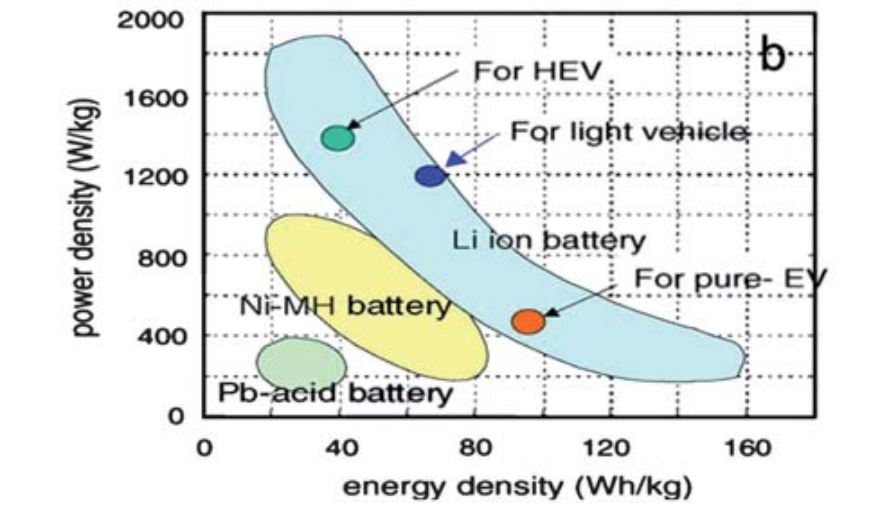
\includegraphics[scale=0.3]{ragone_plot}
	\caption{Plot illustrating the the power and energy densities achievable by three types of battery, as well as the minimum requirements for various types of electric vehicle, including hybrid electric vehicles (HEV), plug in hybrids (light vehicle). From \cite{etacheri_challenges_2011} }
	\label{ragone}
	
\end{figure}
The pursuit of developing new and improved battery materials has shifted the focus of analysis towards studying the microstructure of materials \cite{lu_lithium_2012,arthur_spontaneous_2016, muller_quantification_2018}. The ability to identify crystal structure and composition has become an essential element to understanding and tailoring material properties.  On this front, electron microscopy has become a central technique to this effort  \cite{chiu_aqueous_2013,inkson_2_2016}.  Rapidly improving technology, the possibility of atomic level resolution, coupled with the increasing accessibility have made electron microscopy one of the most prevalent techniques for studying nanoscale features in materials \cite{hansen_atomic-resolution_2001}.  Here, however lithium is at odds with the method.  Novel battery materials are increasingly intricate and lithium's lightness and ionizable nature make it particularly sensitive to electron beams, and often require indirect analysis \cite{kobayashi_quantitative_2017}.  These properties make electron energy loss spectroscopy (EELS), a low dosage technique that is well suited for light elements such as lithium, attractive for battery material analysis  \cite{Egerton}. Recent advances extending EELS into low voltage STEM have made EELS appropriate for a range of new materials \cite{SU_9000}.  However, EELS results are largely qualitative and unstudied systems require a degree of theoretical support.  The theoretical support is all the more essential in dealing with novel technique of low voltage EELS required to study lithium materials with a limited beam life.    
\\
The theoretical support for EELS can come from a number of methods, however, the most prevalent of these are based in density functional theory (DFT), a first principles approach that requires only the locations of atoms in a crystal to determine material properties \cite{ks_1965, wien2k,elk,exciting}.  Here too, results have been limited to qualitative findings, further complicated by lithium's lightweight nature which also poses challenges to theoretical approaches \cite{mauchamp_ab_2006, mauchamp_local_2008}. Much of the challenge in simulating EELS for lithium lies in the treatment of the electron hole created in excited atoms.  Lithium's few core electrons mean that excitonic effects from this hole will always be present in the spectra and current methods in literature lack the subtlety to treat these effects.  The objective of this work is to improve  EELS simulation techniques in order to simulate lithium EELS spectra.  In particular, this work focuses on developing a means to calculate the extent to which the lithium core hole is screened and use these screening calculations to analyze 30keV EELS.  

The outline of this thesis is as follows: in Chapter \ref{literature_review} we will begin with an overview of EELS, DFT and theoretical EELS calculations.  Chapter \ref{methods} will describe the improved method developed in this work, and Chapter \ref{results} will apply the method to a number of lithium materials.  Chapter \ref{conclusion} will conclude the results and address future work.


